\documentclass[xcolor=svgnames]{beamer}
\usepackage{xcolor}
\usepackage{tikz,graphicx}  %图
\usepackage{booktabs}       %三线表\toprule, \midrule, \bottomrule
\usepackage[absolute,overlay]{textpos}
\usepackage{amssymb,amsmath, amssymb,amsbsy, bm}%公式
\usepackage{ctex}
\usepackage{algorithm}
\usepackage{algorithmicx}
\usepackage{algcompatible}
\floatname{algorithm}{\zihao{-5}算法}
\renewcommand{\algorithmicrequire}{\textbf{输入:}}
\renewcommand{\algorithmicensure}{\textbf{输出:}}

\graphicspath{{figures/}}%图片搜索路径
\newcommand{\titlePageLogo}{csu_logo2}%放在首页的logo的图片文件名是csu_logo2,也可以换成其他的
\newcommand{\upRightCornerLogo}{CSU}%放在每一页右上角的logo的文件名是CSU,也可以换成其他的

\usepackage{fontspec}
\setCJKfamilyfont{xw}{STXinwei}%需要STXinwei字体
\newcommand*{\xinwei}{\CJKfamily{xw}}

\mode<presentation>{
\useinnertheme{circles}
\useoutertheme[left,height=0pt,hideothersubsections]{sidebar}


%加入页码和中南大学校徽
\setbeamerfont{footline}{family=\rmfamily, size*={9.3}{5}}
\addtobeamertemplate{background canvas}{}{%
	\usebeamerfont{footline}%
	\usebeamercolor[fg]{new-red}
	\hspace{1em}%
	\tikz[overlay,remember picture] \node[anchor=south east,xshift=0.0pt,yshift=0.001\paperwidth, at=(current page.south east)] {
		\insertframenumber/\inserttotalframenumber};
	\tikz[overlay,remember picture] \node[anchor=north east,xshift=0.0pt,yshift=0.00\paperwidth, opacity=0.65, at=(current page.north east)] {
		\includegraphics[width=0.07\paperwidth]{\upRightCornerLogo}};
}
\setbeamertemplate{navigation symbols}{}%不要导航符

%%%%%%%%%%%%%%%%%%%设置各个元素的字体
\setbeamerfont {title in sidebar}{size*={11.5}{1}, family={\lishu}} %\lishu
%\setbeamerfont{section in sidebar}{size=\scriptsize}
%\setbeamerfont{subsection in sidebar}{size=\tiny,family=\kaishu}
%\setbeamerfont{framesubtitle}{family=\kaishu}
\setbeamerfont{frametitle}{size*={14}{16}, family={\heiti}}
%\setbeamerfont{frametitle}{size=14}
%\setbeamerfont{framesubtitle}{size*={10.5}{12}, family=\heiti}%\heiti}
%\setbeamerfont{framesubtitle}{size*={10.5}{12}, family=\yahei}%\heiti}

\setbeamercovered{transparent}
\setbeamertemplate{blocks}[rounded][shadow=true]


%各种颜色设置
%%%%%%%%%%%%%%%%%%%%%%%%%%%%%%%%%%
\usecolortheme{dolphin}%外部颜色主题
%%%%%%%%%%%%%%%%%%%%%%%%%%%%%%%%%%
%\usecolortheme{spruce}%完整颜色主题
%%%%%%%%%%%%%%%%%%%%%%%%%%%%%%%%%%
\usecolortheme{sidebartab}

\definecolor{new-red}{RGB}{168, 0, 57}
\definecolor{new-red2}{RGB}{153, 0, 0}
\definecolor{new-turquoise}{RGB}{0, 171, 204}
\definecolor{new-blue}{RGB}{45, 122, 180}
\definecolor{new-blue2}{RGB}{51, 102, 153}
\definecolor{new-gray}{RGB}{160, 160, 160}

\setbeamercolor{block title}{fg=new-turquoise,bg=new-gray!30}
\setbeamercolor{section in sidebar}{fg=white, bg=new-gray}
\setbeamercolor{framesubtitle}{fg=FireBrick}
\setbeamercolor{sidebar left}{bg=new-red}


\usefonttheme{serif}
\usefonttheme[onlylarge]{structuresmallcapsserif}
\usefonttheme[onlysmall]{structurebold}

\renewcommand{\raggedright}{\leftskip=0pt \rightskip=0pt plus 0cm}
\raggedright
}




%图标题格式
\usepackage[tableposition=above]{caption}
\setbeamertemplate{caption}{\raggedright\insertcaption\par}
\setbeamertemplate{caption}[numbered]
\DeclareCaptionFont{figurefont}{\kaishu\scriptsize}
\captionsetup{
	labelsep=quad,
	%format=hang,
	labelsep={colon},
	figurename={\kaishu \scriptsize 图},
	tablename={\kaishu \scriptsize 表},
	font=figurefont,
	aboveskip=0.5ex,
	belowskip=-0.5em,
}

\renewcommand{\baselinestretch}{1.5}


\usepackage{natbib}
\bibliographystyle{spbasic}

%================================== 设置英文字体 ================================%
\setmainfont[Mapping=tex-text]{TeX Gyre Pagella}%--------------------------------英文衬线字体
\setsansfont[Mapping=tex-text]{Trebuchet MS}%------------------------------------英文无衬线字体
\setmonofont[Mapping=tex-text]{Courier New}%-------------------------------------英文等宽字体
%\newfontfamily\Arial{Arial}
%================================== 设置英文字体 ================================%

\AtBeginSection[]
{
	{
		\setbeamertemplate{background canvas}{	\usebeamerfont{footline}%
		\usebeamercolor[fg]{frametitle}
		}	
		\begin{frame}<beamer>
		\tableofcontents[sections={2-},currentsection,subsectionstyle=show/show/hide]%,sections={2-6}]
		\end{frame}
	}
	\addtocounter{framenumber}{-1}
}
%\AtBeginSubsection[]
%{
%	{
%		\setbeamertemplate{background canvas}{	\usebeamerfont{footline}%
%			\usebeamercolor[fg]{frametitle}
%		}
%		\begin{frame}<beamer>
%		%\frametitle{提纲}
%		\tableofcontents[sections={2-},currentsection,subsectionstyle=show/shaded/hide]
%		\end{frame}
%	}
%	\addtocounter{framenumber}{-1}
%}





\title[简短标题]{\zihao{-1} \xinwei  这里是大标题}
\author[ZYY]{%
\makebox[4em][s]{\heiti 汇\hspace{\fill}报\hspace{\fill}人}:\makebox[3em][l]{胖虎}\\
\makebox[4em][s]{\heiti 指导老师}:\makebox[3em][l]{牛顿}  \vspace*{3em}}
%\date{2018年9月26日}
\institute% (optional, but mostly needed)
{
  \includegraphics[width=0.7\linewidth]{\titlePageLogo}\\
}


\begin{document}
    \kaishu
	\zihao{-5}
{
	%标题页
	\setbeamertemplate{background canvas}{\usebeamerfont{footline}%
		\usebeamercolor[fg]{frametitle}}
	\begin{frame}
	\titlepage
\end{frame}
\addtocounter{framenumber}{-1}

%%目录	
\section<beamer>*{目录}
\begin{frame}
\frametitle[center]{\Large\bf 目录}
\tableofcontents[sections={2-},hideallsubsections]
%[sectionstyle=show,subsectionstyle=show]
\end{frame}
\addtocounter{framenumber}{-1}
}

\section{理论}
\begin{frame}{帧标题}\framesubtitle{副标题}
输入内容......

输入一个公式,
\begin{equation}
\mathbf{g}(\mathbf{r}')=G\iiint_{\Omega}\frac{\rho dv}{R^2}\frac{\mathbf{r}-\mathbf{r}'}{R}
\end{equation}
\end{frame}

\begin{frame}
总结性文字、概括性文字
\begin{block}{标题}
	\begin{enumerate}
		\item 特点一
		\item 特点二
		\item 特点三
	\end{enumerate}
\end{block}
\end{frame}

\begin{frame}{XXX}
输入一个算法
\begin{algorithm}[H]
	\kaishu\zihao{-5}
	\caption{\zihao{-5}xxx}
\begin{algorithmic}[1]
	\FOR{$n=0$ to $\mathrm{maxit}-1$}
	\STATE $\mathbf{r}_n=\mathbf{G}\mathbf{m}_n-\mathbf{d}$
	\STATE $\mathbf{l}_n=\nabla\phi$
	\STATE ...
	\ENDFOR
\end{algorithmic}
\end{algorithm}
\end{frame}

\section{算例}
\begin{frame}{XXX}
\begin{figure}
	\centering
	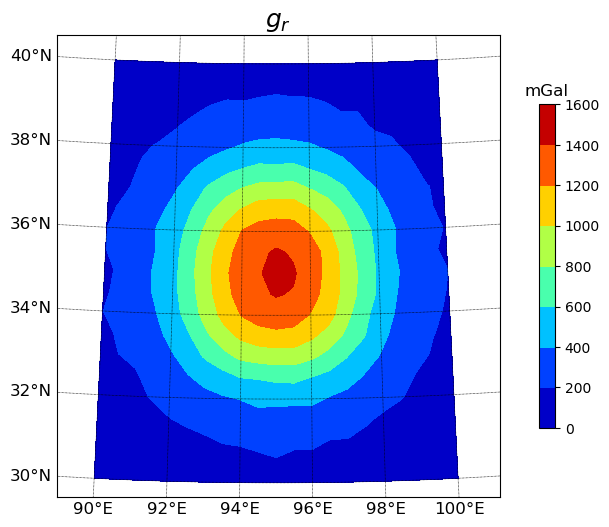
\includegraphics[width=0.65\linewidth]{figures/gr}
	\caption{xxx}
	\label{fig:gr}
\end{figure}
\end{frame}
\begin{frame}{XXX}
\begin{columns}
	\begin{column}{0.4\textwidth}
		左边栏,描述
	\end{column}
	\begin{column}{0.55\textwidth}
		\begin{figure}
			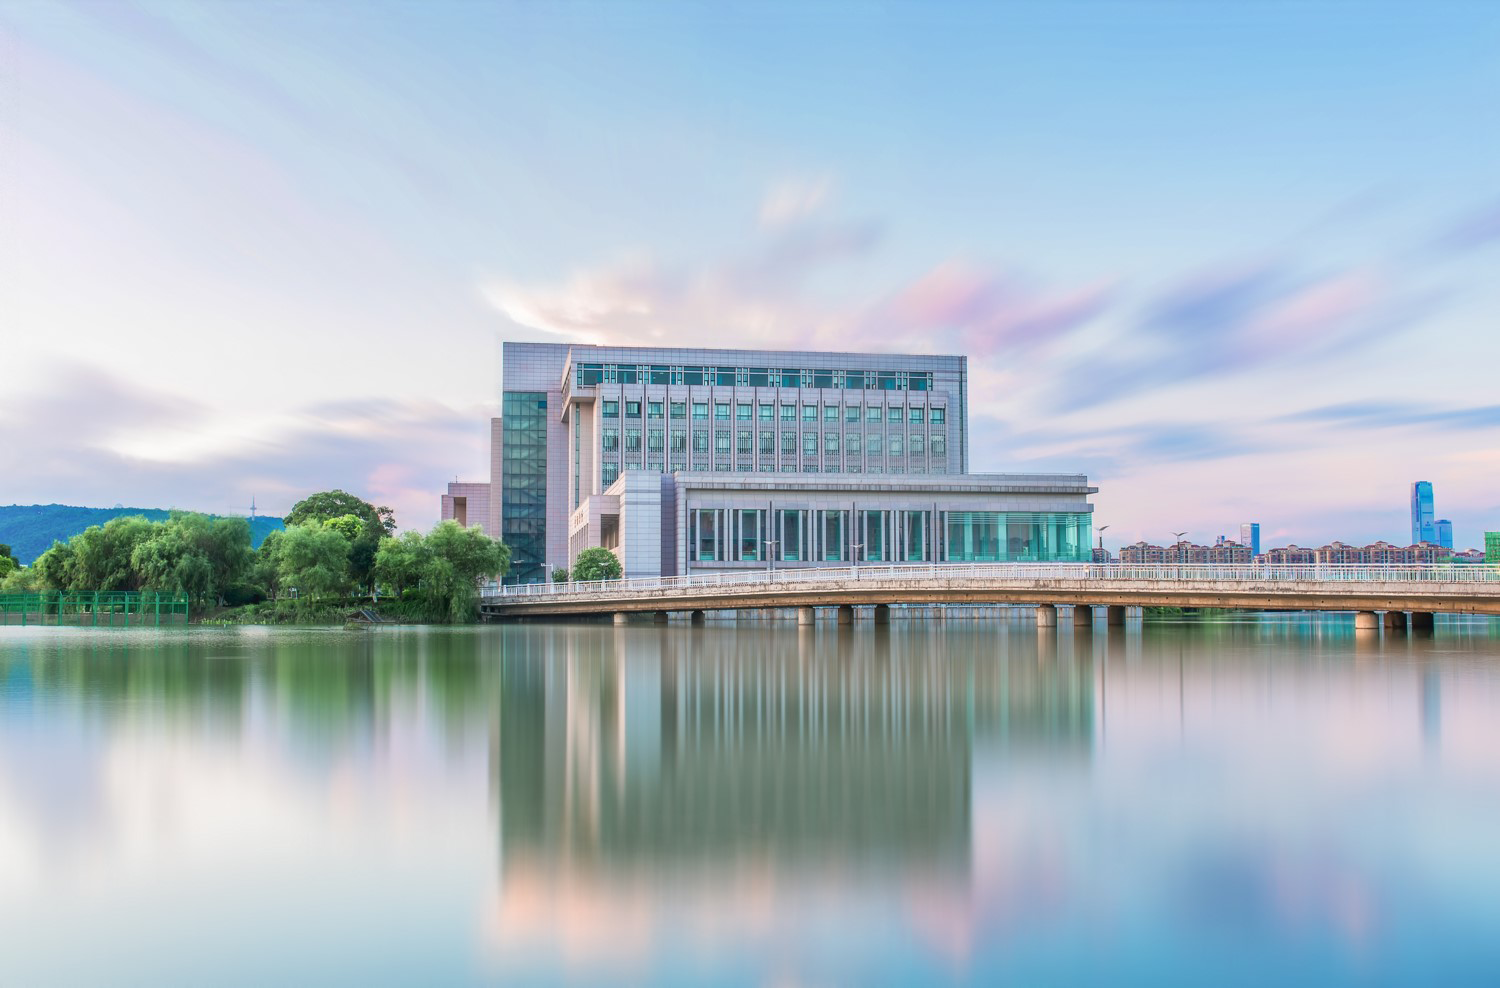
\includegraphics[width=\linewidth]{bg.png}
			\caption{图片}
		\end{figure}
	\end{column}
\end{columns}
\end{frame}

\section{总结}
\begin{frame}{XXX}
\begin{block}{Problems}
	\begin{itemize}
		\item ......
		\item ......
	\end{itemize}
\end{block}
\begin{block}{To do list}
	\begin{itemize}
		\item ......
		\item ......
		\item ......
		\item ......
	\end{itemize}
\end{block}
\end{frame}


%%%%最后致谢页
\usebackgroundtemplate%
{%
	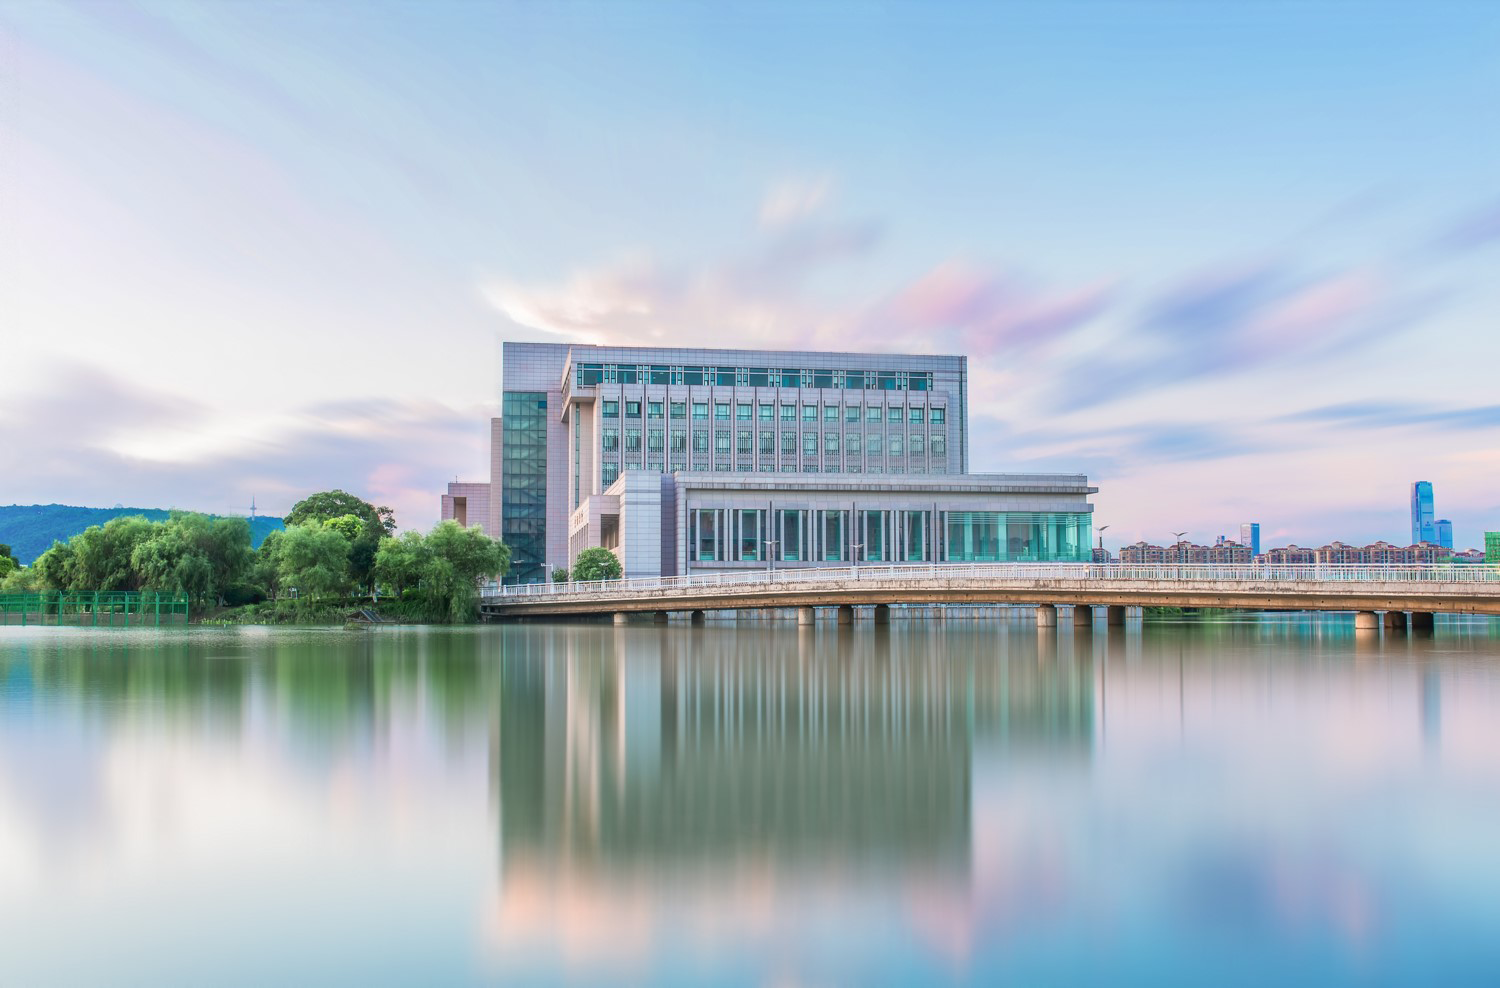
\includegraphics[width=\paperwidth,height=\paperheight]{bg.png}%
}
\begin{frame}
\setbeamercolor{mycolor}{fg=red,bg=white}
\zihao{2}
\begin{beamercolorbox}[rounded=true,shadow=true,wd=\linewidth]{mycolor}
	\xinwei Thank you for your time!
\end{beamercolorbox}
\end{frame}
\addtocounter{framenumber}{-1}
\end{document} 
